
%use mybib.bib for bibliography. bibtex is used for bibliography
\documentclass[journal,12pt,onecolumn]{IEEEtran}
\usepackage[utf8]{inputenc}
\usepackage{graphicx}
\usepackage{cite}
\usepackage{longtable}
\usepackage{amsmath}
\usepackage{multirow}
\usepackage{multicol}
\usepackage{wrapfig}
\usepackage{float}
%\usepackage[section]{placeins}
%\usepackage{subcaption}
\usepackage{array}
\usepackage[export]{adjustbox}
\usepackage{tabu}
\usepackage{tabularx}
\usepackage{listings}
\usepackage{siunitx}
\usepackage{siunitx}
\usepackage{ wasysym }
\usepackage[usenames, dvipsnames]{color}


%%%%%%%%%%%%%%%%%%%%%%%%%%%%%%%%%%%%%%%%%%%%%%%%%%%%%


\ifCLASSINFOpdf

\else

\fi


\hyphenation{op-tical net-works semi-conduc-tor}


\begin{document}

\title{Multiple energy storage}

\author{ Alvi~Newaz,~\IEEEmembership{Student Member,~IEEE,}
Juan~Ospina,~\IEEEmembership{Student Member,~IEEE and}
     Omar~Faruque,~\IEEEmembership{Senior Member,~IEEE}
        }% <-this % stops a space





\maketitle                                                               
\IEEEpeerreviewmaketitle
%\section{Multiple objective A}
With the increase in penetration of Renewable Energy Sources (RES) in the electric distribution network level, it is becoming increasingly difficult to establish stable network operation based on the traditional centralized control scheme of the grid \cite{WHY}. Especially the integration of photovoltaic and wind generation in the low voltage and medium voltage is making the grid less predictable and difficult to control. In general, today's power grid operation is based on day-ahead planning, in which the balancing of demand and generation of the grid is planned to determine optimum set points of operation. In case of a mismatch with the day ahead planning and real scenario a real-time control is usually put in place to take corrective actions \cite{WHY2}. The increasing uncertainty in the grid is resulting in the grid operating sub-optimally based on a day-ahead planned control strategy \cite{WHY2}. To tackle this uncertainty of RES integration, integrating energy storage into the grid has been proposed by several researchers \cite{WHY2,ESI1,ES2,ES3}. 

This document proposes a graph search based control strategy to control multiple energy storage system (ESS). The goal of the control strategy is to provide the most cost optimum operation of the energy storages while providing peak shaving and ramp limiting functionality. In \cite{IM1} the researchers propose a control strategy to smooth out the output of a wind farm using the help of ESS. The control makes sure that the output of the wind farm matches a previously predicted output profile. It optimizes the use of the ESS over a prediction horizon to get better results. In \cite{IM2} researchers optimize ESS connected to a distribution feeder hosting a significant amount of renewable energy resources. The objective of the research is to most cost optimally operate the ESS. Reference \cite{IM3} looks at the optimum use of ESS from a transmission grid standpoint. And the researchers in \cite{IM4} show an IEE 14 bus system based proof of concept of an optimum power flow solution considering ESS. From the discussion thus far it is evident that the integration of RES into the distribution grid is creating some new challenges for grid operation and there has been significant research done to show that ESS can be deployed as a possible solution to counteract the uncertainties introduced to the grid by RES integration. To most optimally control the ESS there needs to be a real-time algorithm which takes into account current and predicted system status \cite{gupta_francis_ospina_newaz_2018}. In case of multiple ESS connected to a distribution system, it is also imperative that the solution obtained does not violate any system constraints \cite{rt4}. So an optimum solution considering both system architecture and constraints and current and predicted system status is necessary to most cost optimally control the ESS while providing necessary services like peak shaving and output ramp rate limiting.


The methodology for solving the problem of optimally controlling the energy storage considering grid constraints and forecasted system status will be developed using a combination of linear programming DC power flow and a graph search solution obtained from the utilization of the A* \cite{a8book} algorithm. The solution will find an optimum and more cost-effective solution to dispatch available energy storage systems in the grid. The solution will take into account not only the present status of the system but also the forecasted values of the grid energy prices, load demand, and generation. The use of the available resources will be optimized by finding the optimum path in a graph search problem formulated to reflect different operation scenarios of the system. Figure \ref{fig:F1_1_Dis} represents a simple example of the graph search formulation of the problem. The values on top of the figure represent the current time step. The values inside the boxes represent the percentage of total energy storage (ES) capacity available in the system. These boxes are the nodes of the graph. The arrows from one box to the next represent the edges of the graph. The values at the bottom of the graph represent the power demand of the system between the current and previous time step. It is assumed that the system power demand is constant between time steps. The system status at T=0 is known from the current measurement. The nodes at T=15, T=30 and T=45 are created based on forecasted values. The target of the solution is to find the most cost optimal path to reach T=45 based on the predictions available. The actual graph formulated will expand 24 hours into the future (T=0 to T=1440) with 15 minute time interval. And the states between the upper and lower limit of the Total energy of the system will be discretized with steps of 2\%.

\begin{figure}[!ht]
\centering
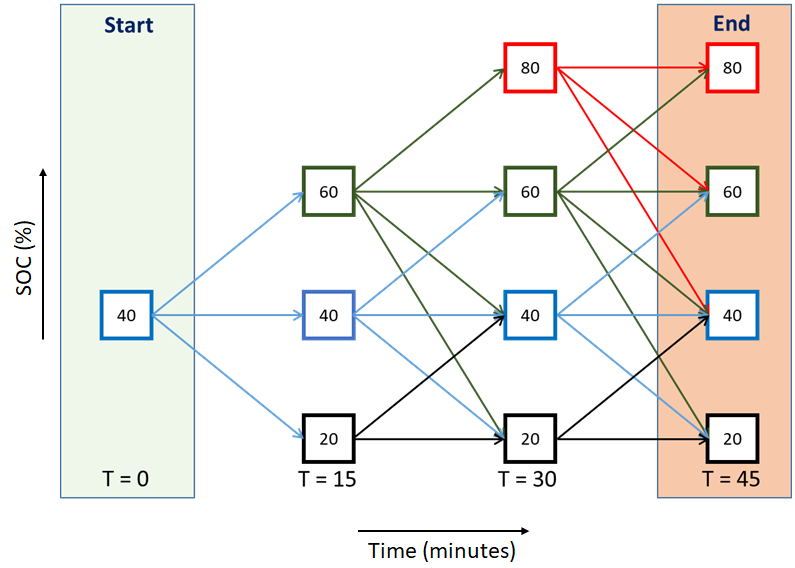
\includegraphics[width = 0.5\linewidth]{figs/F1_1_Dis.png}
\caption{Graph formulation}
\label{fig:F1_1_Dis}
\end{figure}

The cost of the edges is calculated according to equation \ref{eq:COST_FUN}. 
\begin{equation}
\label{eq:COST_FUN}
    C_{total} = E_{grid}*r_{grid} + \sum_{n=1}^{N_{ES}}(E_{ES}(n)*r_{ES}(n))
\end{equation}

Here, $C_{total}$ is the total cost of energy. $E_{grid}$ is the energy drawn from the grid. $R_{grid}$ is the rate of using grid energy. $N_{ES}$ is the total number of energy storage available in the system. $E_{ES}(n)$ and $r_{ES}(n)$ represent the energy usage and the rate of using the $n^{th}$ energy storage. The total energy usage of the energy storages is determined by subtracting the energy at the current node from its parent node. After determining the total energy usage the energy usage is divided between the available energy storages by formulating a linear program to solve the DC optimum power-flow of the grid. Figure \ref{fig:one_line} shows a simplified one-line diagram of an example distribution grid. The grid has 5 buses denoted by the encircled numbers 1,2,3,4 and 5. G denotes the transmission grid. ES1 and ES2 are two energy storages connected to buses 2 and 5. D2, D3, D4 and D5 denotes the demand for the buses 2,3,4 and 5. L1, L2, L3 and L4 represent the maximum power the lines between buses 1 \& 2, 2 \& 3, 3 \& 4 and 4 \& 5 can carry. The impedances of the lines are X1j, X2j, X3j and X4j.
\begin{figure}[!ht]
\centering
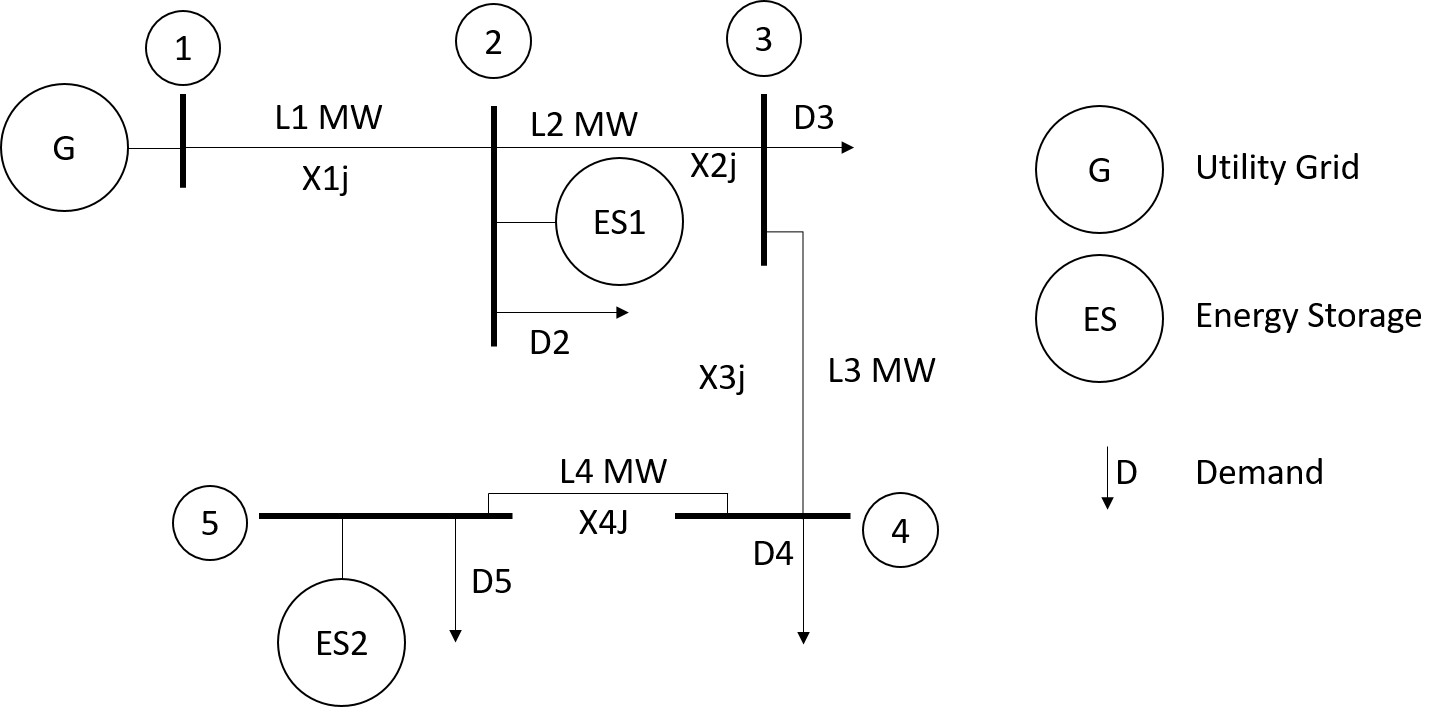
\includegraphics[width = 0.6\linewidth]{{figs/One_line_diagram.png}}
\caption{One-line diagram of simplified distribution system}
\label{fig:one_line}
\end{figure}

A formulation of the linearized economic dispatch problem is shown for this system. Let us assume the total energy difference between the parent and child node of the edge is $\Delta E$. So the total energy supplied by the energy storages $ES1$ and $ES2$ will be $\Delta E$. Let us assume the maximum energy ES1 and ES2 can charge or discharge in between the time steps is $E1_{max}$ and $E2_{max}$. The maximum energy $E1$ and $E2$ can hold are $\overline{E1}$ and $\overline{E2}$ and the minimum energy level $ES1$ and $ES2$ are allowed to be are $\underline{E1}$ and $\underline{E2}$. Taking these values into consideration the economic dispatch problem can be represented as a linear program as follows

Minimize: \\
\begin{equation}
\label{eq:minimize}
    E_{grid}*r_{grid} + E_{ES}(1)*r_{ES}(1) + E_{ES}(2)*r_{ES}(2)
\end{equation}



Subject to: \\
$E_{grid}+ E_{ES}(1)+E_{ES}(2) = D2+D4+D5$ \\
$E_{ES}(1)+E_{ES}(2) = \Delta E$ \\
$-10 \delta_1 + 10 \delta_2 = D2$\\
$-8 \delta_3 + 13 \delta_4 - 5\delta_5 = D4$\\
$-5 \delta_4 + 5 \delta_5 = D5$\\
$10 \delta_1 - 10 \delta_2 \leq L1$\\
$-10 \delta_1 + 10 \delta_2 \leq L1$\\
$5 \delta_2 - 5 \delta_3 \leq L2$\\
$-5 \delta_2 + 5 \delta_3 \leq L2$\\
$8 \delta_2 - 8 \delta_3 \leq L3$\\
$-8 \delta_2 + 8 \delta_3 \leq L3$\\
$5 \delta_4 - 5\delta_5 \leq L4$\\
$-5 \delta_4 + 5\delta_5 \leq L4$\\
$E_{ES}(1) \leq E1_{max}$\\
$E_{ES}(2) \leq E2_{max}$\\
$-E_{ES}(1) \leq E1_{max}$\\
$-E_{ES}(2) \leq E2_{max}$\\
$\underline{E1} \leq ES1_E \leq \overline{E1}$\\
$\underline{E2} \leq ES2_E \leq \overline{E2}$\\

Here, $ES1_E$ and $ES2_E$ are the energy stored by $ES1$ and $ES2$. $\delta_1, \delta_2, \delta_3, \delta_4$ and $\delta_5$ are the angles of busses 1,2,3,4 and 5. The energy values of the grid and ES collected from minimizing equation \ref{eq:minimize} subjected to the mentioned constraints is used in equation \ref{eq:COST_FUN} to get the cost of the edge. After the graph is constructed A* search algorithm is used to find the optimum path to reach different nodes at the end of the time horizon. The end node with the lowest cost is selected as the optimum end node and the algorithm chooses the next best node based on the A* search result to get to that end node. This process is repeated every time step with updated predicted values.

\bibliographystyle{IEEEtran}
\bibliography{mybib.bib}

% \ifCLASSOPTIONcaptionsoff
%   \newpage
% \fi

\end{document}


